\documentclass[journal]{IEEEtran}
\usepackage[caption=false,font=footnotesize]{subfig}
\usepackage{booktabs}
\usepackage{datatool}
\usepackage{listings}
\usepackage{tikz}
\usetikzlibrary{positioning}
\usetikzlibrary{trees}
\usetikzlibrary{fit}
\usetikzlibrary{backgrounds}
\usepackage[hyphens]{url}
\usepackage{hyperref}

\lstdefinestyle{lststyle}{basicstyle=\tt\footnotesize, captionpos=b, frame=single}

\begin{document}
\DTLloaddb{keys_values}{tmp/keys-values.csv}

\title{\LaTeX\ Technical Documents with Docker and Make}

\author{Paschalis~Bizopoulos
\thanks{P. Bizopoulos is an Independent Researcher, Thessaloniki, Greece e-mail: pbizopoulos@protonmail.com}}

\maketitle

\begin{abstract}
	We propose a template for writing portable \LaTeX\ technical documents with Docker and Make in POSIX-oriented operating systems.
	The template provides a Makefile that allows the author to execute the code that generates the variables, tables and figures (results), which are then used during the \LaTeX\ compilation, to produce the fast/draft and slow/final versions of the document.
	We release an open source repository of the template and use it to write this paper.
\end{abstract}

\section{Introduction}
There are multiple ways for writing technical documents that present both computationally generated results (variables, tables and figures) and natural text.
One programming paradigm that tries to solve this task is \textit{literate programming}~\cite{knuth1984literate} in which the author inserts snippets of code and its execution output alongside natural text.
Some applications of \textit{literate programming} include Jupyter~\cite{kluyver2016jupyter} which allows publishing code, results and explanations in a executable format, PythonTeX~\cite{poore2015pythontex} which allows Python to be executed in \LaTeX\ and ActivePapers~\cite{hinsen2014activepapers} in which code can be executed using the Java Virtual Machine.

Although \textit{literate programming} provides many advantages for demonstrative projects and easy visual feedback during experimentation, its `dual nature' makes it difficult to debug and constrains authors in using specific text editors and programming languages thus leading to `app/vendor lock-in` situations.

We propose a template for writing portable \LaTeX\ technical documents with Docker and Make in POSIX-oriented operating systems and provide an open source implementation\footnote{\url{https://github.com/pbizopoulos/latex-technical-documents-with-docker-and-make-template}}.
We write this paper\footnote{\url{https://github.com/pbizopoulos/latex-technical-documents-with-docker-and-make}}\footnote{\url{https://arxiv.org/abs/2005.12660}} using this template and choose the Python programming language~\cite{van2007python} for generating the results.

For the rest of the paper we will refer to:
\begin{itemize}
	\item \textit{results code} as the scientific-oriented programming language code (\textit{main.py}) that produces the variables, tables and figures,
	\item \textit{results} as the variables, tables and figures that are generated by the \textit{results code},
	\item \textit{\LaTeX\ code} as the natural text (\textit{ms.tex}) and bibliography (\textit{ms.bib}),
	\item \textit{code} as both the \textit{\LaTeX\ code} and \textit{results code},
	\item \textit{document} as the technical document that contains the rendered natural text and \textit{results} and
	\item \textit{author} as the author of the \textit{document} that writes and develops the \textit{code}.
\end{itemize}

\section{Template}

\begin{figure}[!t]
	\centering
	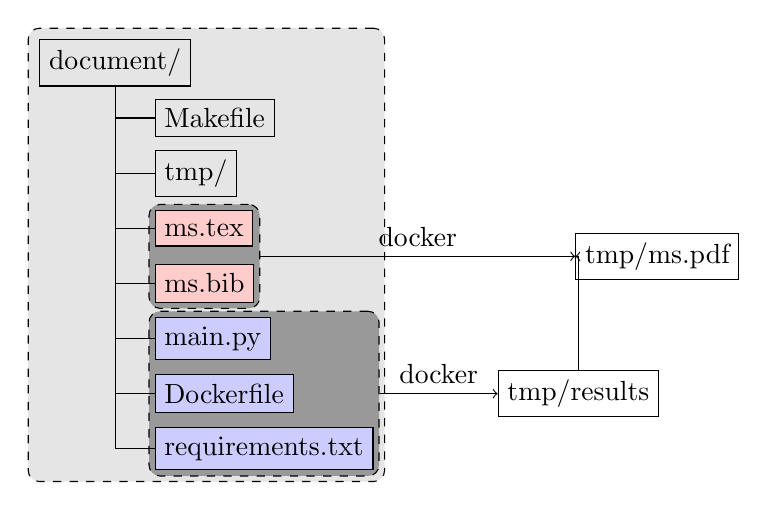
\begin{tikzpicture}[%
			grow via three points={one child at (0.5,-0.7) and two children at (0.5,-0.7) and (0.5,-1.4)},
			edge from parent path={(\tikzparentnode.south) |- (\tikzchildnode.west)}]
			\node[draw](document){document/}
			child{node[draw, anchor=west](makefile){Makefile}}
			child{node[draw, anchor=west](tmp){tmp/}}
			child{node[draw, anchor=west, fill=red!20](tex){ms.tex}}
			child{node[draw, anchor=west, fill=red!20](bib){ms.bib}}
			child{node[draw, anchor=west, fill=blue!20](py){main.py}}
			child{node[draw, anchor=west, fill=blue!20](dockerfile){Dockerfile}}
			child{node[draw, anchor=west, fill=blue!20](requirements){requirements.txt}};
			\begin{scope}[on background layer]
				\node[draw, rounded corners, dashed, fill=gray!20, inner sep=4pt, fit=(document) (requirements)]{};
				\node[draw, rounded corners, dashed, fill=gray!80, inner sep=2pt, fit=(py) (requirements)](code){};
				\node[draw, rounded corners, dashed, fill=gray!80, inner sep=2pt, fit=(tex) (bib)](document){};
			\end{scope}
			\node[draw, right=1.5cm of code, fill=white] (results) {tmp/results};
			\path[draw, ->] (code) -- node[above]{docker} (results);
			\node[draw, right=4cm of document, fill=white] (pdf) {tmp/ms.pdf};
			\path[draw, ->] (results) |- (pdf);
			\path[draw, ->] (document) -- node[above]{docker} (pdf);
	\end{tikzpicture}
	\caption{The file hierarchy of the template is depicted in the light gray background and the arrows denote the data flow towards generating the \textit{document}.
	Blue indicates a \textit{results code} file, red a \textit{\LaTeX\ code} file and within the dark gray background, files that are developed by the \textit{author}.}
	\label{fig:filehierarchyworkflow}
\end{figure}

\LaTeX~\cite{lamport1994latex} is a typesetting system for publishing high quality research documents, and Docker~\cite{merkel2014docker} is a container system that allows portable execution of a codebase between different operating systems/environments.

The proposed template can be used for writing \LaTeX\ \textit{documents} that present \textit{results} generated from \textit{results code} executed within a Docker container.
The file hierarchy of the template is shown in Fig.\ref{fig:filehierarchyworkflow}.

The \textit{author} may use the template for writing \textit{documents} in the following way:
\begin{enumerate}
	\item clones the template,
	\item specifies the name of the \textit{document} in the Makefile,
	\item creates and develops the Dockerfile,
	\item creates and develops the \textit{code} in the local repository including code for:
		\begin{enumerate}
			\item generating fast/draft and slow/final version \textit{document} in \textit{code} and
			\item saving/loading the \textit{results} in/from the \textit{tmp} directory,
		\end{enumerate}
	\item executes \textit{make} for generating the fast/draft version \textit{document} used during development and experimentation,
	\item executes \textit{make ARG=-{}-full} for generating the slow/final version \textit{document} used for distribution and
	\item executes \textit{make clean} to restore to a clean state by removing the \textit{tmp} directory.
\end{enumerate}

The fast/draft version \textit{document} helps in faster iterations during writing and experimentation.
An example of creating a fast/draft version in the field of neural networks is setting the number of epochs and number of training samples to a low value.

The template makes use of the automatic generation of intermediate files of the Make program.
The \textit{author} only needs to edit a file from \textit{results code} or \textit{\LaTeX\ code} and the corresponding compilation is automatically triggered with Make.
Forced compilations without change could be done using the \textit{touch} POSIX utility that updates the modification time.

\section{Template utilities}

A useful \LaTeX\ package for automatically presenting variables from \textit{results} in \textit{\LaTeX\ code} is \textit{datatool} with the following example use:
\begin{lstlisting}[language=TeX, style=lststyle, caption={\LaTeX\ datatool example of loading a file that contains pairs of keys and values (tmp/keys\_values.csv) generated by a \textit{results code} and getting the value of a key named lr.}]
\DTLloaddb{keys_values}{tmp/keys_values.csv}
\DTLfetch{keys_values}{key}{lr}{value}
\end{lstlisting}

Another useful function when using Python for \textit{results code} is \textit{pandas.DataFrame.to\_latex} which automatically converts a dataframe table to a \LaTeX\ table (as shown in Table~\ref{table:table}).
\begin{lstlisting}[language=python, style=lststyle, caption={Convert Pandas DataFrame to \LaTeX\ table.}]
df = pd.DataFrame(table)
df.to_latex("tmp/metrics.tex", float_format="%.2f")
\end{lstlisting}

Regarding \LaTeX\ a culprit against reproducibility is the time-date metadata embedded in the pdf output.
These can be disabled using the following commands into the \textit{\LaTeX\ code} or as extra arguments during \LaTeX\ compilation (as done in the template Makefile):
\begin{lstlisting}[language=TeX, style=lststyle, caption={\LaTeX\ pdf reproducibility commands.}]
\pdfinfoomitdate=1
\pdfsuppressptexinfo=-1
\pdftrailerid{}
\end{lstlisting}

Regarding the \textit{results code} for Python, random seeds need to be set to a specific value such as:
\begin{lstlisting}[language=python, style=lststyle, caption={Python reproducibility commands for some popular libraries.}]
# for build-in random module
random.seed(0)
# for numpy
np.random.seed(0)
# for tensorflow
tf.random.set_seed(0)
# for pytorch
torch.backends.cudnn.benchmark = False
torch.backends.cudnn.deterministic = True
torch.cuda.manual_seed_all(0)
torch.manual_seed(0)
\end{lstlisting}

Setting the random seeds and the previously mentioned \LaTeX\ packages we could have deterministic stochasticity that generates variables, tables and figures.

An \textit{author} can use the POSIX utility \textit{cmp} to compare \textit{documents} (generated in a different session, OS or underlying hardware) byte by byte, and diffoscope\footnote{\url{https://diffoscope.org/}} for identifying sources of non-determinism as follows:
\begin{lstlisting}[language=bash, style=lststyle, caption={Test fast/draft document reproducibility.}]
# Generate the first fast/draft document version
make
# Backup the first resulting pdf
cp tmp/ms.pdf tmp/ms-previous.pdf
# Update the modification timestamp of main.py
touch main.py
# Generate the second fast/draft document version
make
# Compare fast/draft document versions byte by byte
cmp tmp/ms.pdf tmp/ms-previous.pdf
# Compare fast/draft document versions
# in a human readable form
diffoscope tmp/ms.pdf tmp/ms-previous.pdf
\end{lstlisting}

\section{Example use case of the template}
This sections provides a use case of the template and also serves as a manual for writing \LaTeX\ \textit{documents} with Python as the \textit{results code} programming language.
We train and test a MobilenetV2 neural network~\cite{sandler2018mobilenetv2} in PyTorch~\cite{paszke2019pytorch}, on the following datasets:
\begin{itemize}
	\item MNIST~\cite{lecun2010mnist},
	\item FashionMNIST~\cite{xiao2017fashion},
	\item KMNIST~\cite{clanuwat2018deep},
	\item CIFAR10~\cite{krizhevsky2009learning},
	\item CIFAR100~\cite{krizhevsky2009learning} and
	\item SVHN~\cite{netzer2011reading}.
\end{itemize}

We use the default train, validation and test datasets and compare the use of ReLU6\cite{dahl2013improving} and SiLU\cite{elfwing2018sigmoid} activation functions in a VGG11 model.
The images from the MNIST variants are resized to $32\times 32$ to comply with the dimensions of VGG11.

Making use of the \textit{datatool} package the values of the following variables are not referred in the main \textit{.tex} file but they are read by an intermediate \textit{.tex} file created by the \textit{results code}:
\begin{itemize}
	\item the number of epochs is $\DTLfetch{keys_values}{key}{num_epochs}{value}$,
	\item the batch size is $\DTLfetch{keys_values}{key}{batch_size}{value}$ and
	\item the learning rate for SGD is $\DTLfetch{keys_values}{key}{lr}{value}$.
\end{itemize}

Making use of setting the random seeds we consistenly get the same figures as shown in Fig.\ref{fig:image} which depicts the train and validation loss for all datasets.
\begin{figure}[!t]
	\subfloat{\includegraphics[width=0.25\textwidth]{tmp/MNIST-loss.pdf}}
	\subfloat{\includegraphics[width=0.25\textwidth]{tmp/FashionMNIST-loss.pdf}}
	\\
	\subfloat{\includegraphics[width=0.25\textwidth]{tmp/KMNIST-loss.pdf}}
	\subfloat{\includegraphics[width=0.25\textwidth]{tmp/CIFAR10-loss.pdf}}
	\\
	\subfloat{\includegraphics[width=0.25\textwidth]{tmp/CIFAR100-loss.pdf}}
	\subfloat{\includegraphics[width=0.25\textwidth]{tmp/SVHN-loss.pdf}}
	\caption{Comparison of ReLU6 and SiLU train and validation losses for all datasets.}
	\label{fig:image}
\end{figure}

\begin{table}[h]
	\centering
	\caption{Table example created from results code.}
	\label{table:table}
	\setlength\tabcolsep{2pt}
	\input{tmp/metrics.tex}
\end{table}

\section{Discussion}
The proposed template is based on plain text files and can be used with any POSIX-oriented operating that supports Docker and Make.
Moreover it can be combined with any version control system, docker container registry providor and text editor thus preventing `app/vendor lock-in' situations.

Potential uses of the template include:
\begin{itemize}
	\item regression testing and debugging, to ensure that changes to \textit{code} do not alter the results.
	\item common environment across multiple \textit{authors},
	\item reviewer, coauthor(s), journal editors or other researchers can easily reproduce the \textit{document} with minimal requirements.
\end{itemize}

\section{Conclusion}
Creation, usage and publication of technical documents are one of the top challenges for reproducible technical documents~\cite{barba2019praxis}.
The proposed template aids to this purpose in writing reproducible technical documents using the tools that most of academics already use (\LaTeX, Docker, Make) in a portable and efficient way.

\bibliographystyle{IEEEtran}
\bibliography{ms.bib}

\end{document}
